\section{圆柱体}\label{sec:圆柱体}

另一个有用的二次曲面是\keyindex{圆柱体}{cylinder}{};
pbrt提供以$z$轴为中心的圆柱体\refvar{Shape}{}。
实现在文件\href{https://github.com/mmp/pbrt-v3/tree/master/src/shapes/cylinder.h}{\ttfamily shapes/cylinder.h}和
\href{https://github.com/mmp/pbrt-v3/tree/master/src/shapes/cylinder.cpp}{\ttfamily shapes/cylinder.cpp}内。
用户为圆柱体提供最小和最大$z$值,以及半径和最大扫掠值$\varphi$(\reffig{3.6})。
\begin{figure}[htbp]
    \centering%LaTeX with PSTricks extensions
%%Creator: Inkscape 1.0.1 (3bc2e813f5, 2020-09-07)
%%Please note this file requires PSTricks extensions
\psset{xunit=.35pt,yunit=.35pt,runit=.35pt}
\begin{pspicture}(448.67001343,346.17999268)
{
\newrgbcolor{curcolor}{0.50196081 0.50196081 0.50196081}
\pscustom[linewidth=1,linecolor=curcolor]
{
\newpath
\moveto(247.69,277.90999268)
\curveto(247.69,272.81999268)(231.64,268.68999268)(211.84,268.68999268)
\curveto(192.04,268.68999268)(176,272.81999268)(176,277.90999268)
\curveto(176,282.99999268)(192.05,287.12999268)(211.84,287.12999268)
\curveto(222.98,287.12999268)(232.93,285.82999268)(239.5,283.77999268)
}
}
{
\newrgbcolor{curcolor}{0 0 0}
\pscustom[linewidth=1,linecolor=curcolor]
{
\newpath
\moveto(211.83000183,101.72999573)
\lineto(211.83000183,314.95999336)
}
}
{
\newrgbcolor{curcolor}{0 0 0}
\pscustom[linestyle=none,fillstyle=solid,fillcolor=curcolor]
{
\newpath
\moveto(217.34,310.04999268)
\lineto(211.83,314.30999268)
\lineto(206.33,310.04999268)
\lineto(211.83,323.05999268)
\closepath
}
}
{
\newrgbcolor{curcolor}{0.65098041 0.65098041 0.65098041}
\pscustom[linestyle=none,fillstyle=solid,fillcolor=curcolor]
{
\newpath
\moveto(216.13,311.60999268)
\lineto(211.83,321.74999268)
\lineto(211.83,314.93999268)
\closepath
}
}
{
\newrgbcolor{curcolor}{0.40000001 0.40000001 0.40000001}
\pscustom[linestyle=none,fillstyle=solid,fillcolor=curcolor]
{
\newpath
\moveto(207.53,311.60999268)
\lineto(211.83,321.74999268)
\lineto(211.83,314.93999268)
\closepath
}
}
{
\newrgbcolor{curcolor}{0 0 0}
\pscustom[linewidth=1,linecolor=curcolor]
{
\newpath
\moveto(211.83000183,102.07998657)
\lineto(132.74000549,23.97998047)
}
}
{
\newrgbcolor{curcolor}{0 0 0}
\pscustom[linestyle=none,fillstyle=solid,fillcolor=curcolor]
{
\newpath
\moveto(132.37,31.34999268)
\lineto(133.2,24.43999268)
\lineto(140.1,23.50999268)
\lineto(126.97,18.28999268)
\closepath
}
}
{
\newrgbcolor{curcolor}{0.65098041 0.65098041 0.65098041}
\pscustom[linestyle=none,fillstyle=solid,fillcolor=curcolor]
{
\newpath
\moveto(132.1,29.38999268)
\lineto(127.91,19.20999268)
\lineto(132.75,23.98999268)
\closepath
}
}
{
\newrgbcolor{curcolor}{0.40000001 0.40000001 0.40000001}
\pscustom[linestyle=none,fillstyle=solid,fillcolor=curcolor]
{
\newpath
\moveto(138.14,23.27999268)
\lineto(127.91,19.20999268)
\lineto(132.75,23.98999268)
\closepath
}
}
{
\newrgbcolor{curcolor}{0 0 0}
\pscustom[linewidth=1,linecolor=curcolor]
{
\newpath
\moveto(211.57000732,102.31999207)
\lineto(424.79998779,102.31999207)
}
}
{
\newrgbcolor{curcolor}{0 0 0}
\pscustom[linestyle=none,fillstyle=solid,fillcolor=curcolor]
{
\newpath
\moveto(419.89,96.80999268)
\lineto(424.15,102.31999268)
\lineto(419.89,107.81999268)
\lineto(432.91,102.31999268)
\closepath
}
}
{
\newrgbcolor{curcolor}{0.65098041 0.65098041 0.65098041}
\pscustom[linestyle=none,fillstyle=solid,fillcolor=curcolor]
{
\newpath
\moveto(421.45,98.01999268)
\lineto(431.59,102.31999268)
\lineto(424.78,102.31999268)
\closepath
}
}
{
\newrgbcolor{curcolor}{0.40000001 0.40000001 0.40000001}
\pscustom[linestyle=none,fillstyle=solid,fillcolor=curcolor]
{
\newpath
\moveto(421.45,106.61999268)
\lineto(431.59,102.31999268)
\lineto(424.78,102.31999268)
\closepath
}
}
{
\newrgbcolor{curcolor}{0 0 0}
\pscustom[linewidth=1,linecolor=curcolor]
{
\newpath
\moveto(350.83000183,277.73999023)
\curveto(350.83000183,286.35502645)(316.96111637,294.12183088)(265.01762877,297.41847591)
\curveto(213.07424711,300.71511422)(153.28645653,298.89232333)(113.53009079,292.80059904)
\curveto(73.77372505,286.70887475)(61.87766115,277.5478076)(83.39248224,269.58871089)
\curveto(104.90734722,261.62959795)(155.59577355,256.439991)(211.82000732,256.439991)
\curveto(268.0442411,256.439991)(318.73266743,261.62959795)(340.2475324,269.58871089)
\curveto(361.7623535,277.5478076)(349.86628959,286.70887475)(310.10992386,292.80059904)
\curveto(270.35355812,298.89232333)(210.56576754,300.71511422)(158.62238587,297.41847591)
\curveto(106.67889828,294.12183088)(72.81001282,286.35502645)(72.81001282,277.73999023)
\curveto(72.81001282,269.12495402)(106.67889828,261.35814959)(158.62238587,258.06150455)
\curveto(210.56576754,254.76486625)(270.35355812,256.58765714)(310.10992386,262.67938143)
\curveto(349.86628959,268.77110572)(361.7623535,277.93217287)(340.2475324,285.89126957)
\curveto(318.73266743,293.85038252)(268.0442411,299.03998947)(211.82000732,299.03998947)
\curveto(155.59577355,299.03998947)(104.90734722,293.85038252)(83.39248224,285.89126957)
\curveto(61.87766115,277.93217287)(73.77372505,268.77110572)(113.53009079,262.67938143)
\curveto(153.28645653,256.58765714)(213.07424711,254.76486625)(265.01762877,258.06150455)
\curveto(316.96111637,261.35814959)(350.83000183,269.12495402)(350.83000183,277.73999023)
\closepath
}
}
{
\newrgbcolor{curcolor}{0 0 0}
\pscustom[linewidth=1,linecolor=curcolor]
{
\newpath
\moveto(211.74000549,278.00999451)
\lineto(291.57000732,295.15999222)
}
}
{
\newrgbcolor{curcolor}{0 0 0}
\pscustom[linewidth=1,linecolor=curcolor]
{
\newpath
\moveto(211.88999939,278.00999451)
\lineto(350.79000854,278.00999451)
}
}
{
\newrgbcolor{curcolor}{0 0 0}
\pscustom[linewidth=1,linecolor=curcolor]
{
\newpath
\moveto(350.72999573,140.75)
\curveto(350.72999573,149.36503621)(316.86111027,157.13184065)(264.91762267,160.42848568)
\curveto(212.97424101,163.72512399)(153.18645043,161.90233309)(113.43008469,155.8106088)
\curveto(73.67371895,149.71888452)(61.77765504,140.55781737)(83.29247614,132.59872066)
\curveto(104.80734112,124.63960772)(155.49576745,119.45000076)(211.72000122,119.45000076)
\curveto(267.94423499,119.45000076)(318.63266133,124.63960772)(340.1475263,132.59872066)
\curveto(361.6623474,140.55781737)(349.76628349,149.71888452)(310.00991775,155.8106088)
\curveto(270.25355201,161.90233309)(210.46576143,163.72512399)(158.52237977,160.42848568)
\curveto(106.57889217,157.13184065)(72.71000671,149.36503621)(72.71000671,140.75)
\curveto(72.71000671,132.13496379)(106.57889217,124.36815935)(158.52237977,121.07151432)
\curveto(210.46576143,117.77487601)(270.25355201,119.59766691)(310.00991775,125.6893912)
\curveto(349.76628349,131.78111548)(361.6623474,140.94218263)(340.1475263,148.90127934)
\curveto(318.63266133,156.86039228)(267.94423499,162.04999924)(211.72000122,162.04999924)
\curveto(155.49576745,162.04999924)(104.80734112,156.86039228)(83.29247614,148.90127934)
\curveto(61.77765504,140.94218263)(73.67371895,131.78111548)(113.43008469,125.6893912)
\curveto(153.18645043,119.59766691)(212.97424101,117.77487601)(264.91762267,121.07151432)
\curveto(316.86111027,124.36815935)(350.72999573,132.13496379)(350.72999573,140.75)
\closepath
}
}
{
\newrgbcolor{curcolor}{0 0 0}
\pscustom[linewidth=1,linecolor=curcolor]
{
\newpath
\moveto(72.76999664,277.96999359)
\lineto(72.76999664,140.83999634)
}
}
{
\newrgbcolor{curcolor}{0 0 0}
\pscustom[linewidth=1,linecolor=curcolor]
{
\newpath
\moveto(350.79998779,278.11999512)
\lineto(350.79998779,140.22999573)
}
}
{
\newrgbcolor{curcolor}{0 0 0}
\pscustom[linewidth=1,linecolor=curcolor]
{
\newpath
\moveto(68.01000214,140.95999146)
\lineto(33.52000046,140.95999146)
}
}
{
\newrgbcolor{curcolor}{0 0 0}
\pscustom[linewidth=1,linecolor=curcolor]
{
\newpath
\moveto(68.01000214,277.78999329)
\lineto(33.52000046,277.78999329)
}
}
{
\newrgbcolor{curcolor}{0 0 0}
\pscustom[linestyle=none,fillstyle=solid,fillcolor=curcolor]
{
\newpath
\moveto(282.46993563,265.46999408)
\curveto(282.39181063,265.07936908)(282.23556063,264.49343158)(282.23556063,264.37624408)
\curveto(282.23556063,263.94655658)(282.58712313,263.71218158)(282.97774813,263.71218158)
\curveto(283.29024813,263.71218158)(283.71993563,263.90749408)(283.91524813,264.41530658)
\curveto(283.95431063,264.49343158)(284.77462313,267.89186908)(284.89181063,268.36061908)
\curveto(285.08712313,269.18093158)(285.55587313,270.89968158)(285.67306063,271.60280658)
\curveto(285.79024813,271.91530658)(286.49337313,273.08718158)(287.07931063,273.63405658)
\curveto(287.27462313,273.79030658)(288.01681063,274.45436908)(289.07149813,274.45436908)
\curveto(289.73556063,274.45436908)(290.08712313,274.14186908)(290.12618563,274.14186908)
\curveto(289.38399813,274.02468158)(288.83712313,273.43874408)(288.83712313,272.77468158)
\curveto(288.83712313,272.38405658)(289.11056063,271.91530658)(289.77462313,271.91530658)
\curveto(290.43868563,271.91530658)(291.14181063,272.50124408)(291.14181063,273.39968158)
\curveto(291.14181063,274.25905658)(290.36056063,275.00124408)(289.07149813,275.00124408)
\curveto(287.46993563,275.00124408)(286.37618563,273.79030658)(285.90743563,273.08718158)
\curveto(285.67306063,274.21999408)(284.77462313,275.00124408)(283.60274813,275.00124408)
\curveto(282.46993563,275.00124408)(282.00118563,274.02468158)(281.76681063,273.59499408)
\curveto(281.33712313,272.73561908)(281.02462313,271.25124408)(281.02462313,271.17311908)
\curveto(281.02462313,270.89968158)(281.25899813,270.89968158)(281.29806063,270.89968158)
\curveto(281.57149813,270.89968158)(281.57149813,270.93874408)(281.72774813,271.48561908)
\curveto(282.15743563,273.24343158)(282.66524813,274.45436908)(283.56368563,274.45436908)
\curveto(283.95431063,274.45436908)(284.30587313,274.25905658)(284.30587313,273.32155658)
\curveto(284.30587313,272.77468158)(284.22774813,272.50124408)(283.91524813,271.21218158)
\closepath
\moveto(282.46993563,265.46999408)
}
}
{
\newrgbcolor{curcolor}{0 0 0}
\pscustom[linestyle=none,fillstyle=solid,fillcolor=curcolor]
{
\newpath
\moveto(442.23157013,104.08531158)
\curveto(442.38782013,104.71031158)(442.97375763,107.01499908)(444.69250763,107.01499908)
\curveto(444.80969513,107.01499908)(445.43469513,107.01499908)(445.94250763,106.70249908)
\curveto(445.23938263,106.54624908)(444.77063263,105.96031158)(444.77063263,105.33531158)
\curveto(444.77063263,104.94468658)(445.04407013,104.47593658)(445.70813263,104.47593658)
\curveto(446.25500763,104.47593658)(447.03625763,104.90562408)(447.03625763,105.92124908)
\curveto(447.03625763,107.21031158)(445.59094513,107.56187408)(444.73157013,107.56187408)
\curveto(443.28625763,107.56187408)(442.42688263,106.23374908)(442.11438263,105.68687408)
\curveto(441.48938263,107.32749908)(440.16125763,107.56187408)(439.41907013,107.56187408)
\curveto(436.84094513,107.56187408)(435.39563263,104.35874908)(435.39563263,103.73374908)
\curveto(435.39563263,103.46031158)(435.66907013,103.46031158)(435.70813263,103.46031158)
\curveto(435.90344513,103.46031158)(435.98157013,103.53843658)(436.02063263,103.73374908)
\curveto(436.88000763,106.38999908)(438.52063263,107.01499908)(439.38000763,107.01499908)
\curveto(439.84875763,107.01499908)(440.70813263,106.78062408)(440.70813263,105.33531158)
\curveto(440.70813263,104.55406158)(440.27844513,102.91343658)(439.38000763,99.39781158)
\curveto(438.98938263,97.87437408)(438.09094513,96.81968658)(436.99719513,96.81968658)
\curveto(436.84094513,96.81968658)(436.29407013,96.81968658)(435.74719513,97.13218658)
\curveto(436.37219513,97.28843658)(436.91907013,97.79624908)(436.91907013,98.49937408)
\curveto(436.91907013,99.16343658)(436.37219513,99.35874908)(436.02063263,99.35874908)
\curveto(435.23938263,99.35874908)(434.65344513,98.73374908)(434.65344513,97.91343658)
\curveto(434.65344513,96.78062408)(435.86438263,96.27281158)(436.95813263,96.27281158)
\curveto(438.63782013,96.27281158)(439.53625763,98.03062408)(439.57532013,98.14781158)
\curveto(439.88782013,97.24937408)(440.78625763,96.27281158)(442.27063263,96.27281158)
\curveto(444.84875763,96.27281158)(446.25500763,99.47593658)(446.25500763,100.10093658)
\curveto(446.25500763,100.37437408)(446.05969513,100.37437408)(445.98157013,100.37437408)
\curveto(445.74719513,100.37437408)(445.70813263,100.25718658)(445.63000763,100.10093658)
\curveto(444.80969513,97.40562408)(443.13000763,96.81968658)(442.34875763,96.81968658)
\curveto(441.37219513,96.81968658)(440.98157013,97.60093658)(440.98157013,98.46031158)
\curveto(440.98157013,99.00718658)(441.09875763,99.55406158)(441.37219513,100.64781158)
\closepath
\moveto(442.23157013,104.08531158)
}
}
{
\newrgbcolor{curcolor}{0 0 0}
\pscustom[linestyle=none,fillstyle=solid,fillcolor=curcolor]
{
\newpath
\moveto(124.36640263,18.72960658)
\curveto(124.48359013,19.08116908)(124.48359013,19.12023158)(124.48359013,19.31554408)
\curveto(124.48359013,19.74523158)(124.13202763,19.97960658)(123.74140263,19.97960658)
\curveto(123.50702763,19.97960658)(123.11640263,19.82335658)(122.88202763,19.47179408)
\curveto(122.84296513,19.31554408)(122.60859013,18.57335658)(122.53046513,18.10460658)
\curveto(122.33515263,17.47960658)(122.17890263,16.77648158)(122.02265263,16.11241908)
\lineto(120.88984013,11.62023158)
\curveto(120.81171513,11.26866908)(119.71796513,9.51085658)(118.07734013,9.51085658)
\curveto(116.82734013,9.51085658)(116.55390263,10.60460658)(116.55390263,11.54210658)
\curveto(116.55390263,12.67491908)(116.98359013,14.23741908)(117.80390263,16.42491908)
\curveto(118.19452763,17.44054408)(118.31171513,17.71398158)(118.31171513,18.22179408)
\curveto(118.31171513,19.31554408)(117.53046513,20.25304408)(116.28046513,20.25304408)
\curveto(113.89765263,20.25304408)(112.99921513,16.62023158)(112.99921513,16.42491908)
\curveto(112.99921513,16.15148158)(113.23359013,16.15148158)(113.27265263,16.15148158)
\curveto(113.54609013,16.15148158)(113.54609013,16.22960658)(113.66327763,16.62023158)
\curveto(114.36640263,18.96398158)(115.34296513,19.70616908)(116.20234013,19.70616908)
\curveto(116.39765263,19.70616908)(116.82734013,19.70616908)(116.82734013,18.92491908)
\curveto(116.82734013,18.29991908)(116.55390263,17.63585658)(116.39765263,17.16710658)
\curveto(115.38202763,14.51085658)(114.95234013,13.10460658)(114.95234013,11.93273158)
\curveto(114.95234013,9.70616908)(116.51484013,8.96398158)(117.99921513,8.96398158)
\curveto(118.97577763,8.96398158)(119.79609013,9.39366908)(120.49921513,10.09679408)
\curveto(120.18671513,8.80773158)(119.87421513,7.55773158)(118.89765263,6.22960658)
\curveto(118.23359013,5.40929408)(117.29609013,4.66710658)(116.16327763,4.66710658)
\curveto(115.81171513,4.66710658)(114.67890263,4.74523158)(114.24921513,5.72179408)
\curveto(114.63984013,5.72179408)(114.99140263,5.72179408)(115.30390263,6.03429408)
\curveto(115.57734013,6.22960658)(115.81171513,6.58116908)(115.81171513,7.04991908)
\curveto(115.81171513,7.83116908)(115.14765263,7.90929408)(114.91327763,7.90929408)
\curveto(114.32734013,7.90929408)(113.50702763,7.51866908)(113.50702763,6.30773158)
\curveto(113.50702763,5.05773158)(114.60077763,4.12023158)(116.16327763,4.12023158)
\curveto(118.70234013,4.12023158)(121.28046513,6.38585658)(121.98359013,9.19835658)
\closepath
\moveto(124.36640263,18.72960658)
}
}
{
\newrgbcolor{curcolor}{0 0 0}
\pscustom[linestyle=none,fillstyle=solid,fillcolor=curcolor]
{
\newpath
\moveto(208.32254713,328.08682158)
\curveto(209.65067213,329.53213408)(210.39285963,330.15713408)(211.29129713,330.93838408)
\curveto(211.29129713,330.93838408)(212.81473463,332.26650908)(213.71317213,333.16494658)
\curveto(216.09598463,335.46963408)(216.64285963,336.68057158)(216.64285963,336.79775908)
\curveto(216.64285963,337.03213408)(216.40848463,337.03213408)(216.36942213,337.03213408)
\curveto(216.17410963,337.03213408)(216.13504713,336.99307158)(215.97879713,336.75869658)
\curveto(215.23660963,335.54775908)(214.72879713,335.15713408)(214.14285963,335.15713408)
\curveto(213.51785963,335.15713408)(213.24442213,335.54775908)(212.85379713,335.97744658)
\curveto(212.38504713,336.52432158)(211.95535963,337.03213408)(211.13504713,337.03213408)
\curveto(209.26004713,337.03213408)(208.12723463,334.72744658)(208.12723463,334.18057158)
\curveto(208.12723463,334.06338408)(208.20535963,333.90713408)(208.40067213,333.90713408)
\curveto(208.63504713,333.90713408)(208.67410963,334.02432158)(208.75223463,334.18057158)
\curveto(209.22098463,335.35244658)(210.66629713,335.35244658)(210.86160963,335.35244658)
\curveto(211.36942213,335.35244658)(211.83817213,335.19619658)(212.42410963,335.00088408)
\curveto(213.43973463,334.61025908)(213.71317213,334.61025908)(214.33817213,334.61025908)
\curveto(213.43973463,333.55557158)(211.36942213,331.75869658)(210.90067213,331.36807158)
\lineto(208.63504713,329.25869658)
\curveto(206.95535963,327.57900908)(206.05692213,326.17275908)(206.05692213,325.97744658)
\curveto(206.05692213,325.74307158)(206.33035963,325.74307158)(206.36942213,325.74307158)
\curveto(206.56473463,325.74307158)(206.60379713,325.78213408)(206.76004713,326.05557158)
\curveto(207.34598463,326.95400908)(208.08817213,327.61807158)(208.90848463,327.61807158)
\curveto(209.45535963,327.61807158)(209.72879713,327.38369658)(210.35379713,326.68057158)
\curveto(210.74442213,326.13369658)(211.21317213,325.74307158)(211.91629713,325.74307158)
\curveto(214.41629713,325.74307158)(215.86160963,328.90713408)(215.86160963,329.57119658)
\curveto(215.86160963,329.68838408)(215.74442213,329.84463408)(215.54910963,329.84463408)
\curveto(215.31473463,329.84463408)(215.27567213,329.68838408)(215.19754713,329.49307158)
\curveto(214.61160963,327.89150908)(213.01004713,327.42275908)(212.18973463,327.42275908)
\curveto(211.72098463,327.42275908)(211.25223463,327.57900908)(210.74442213,327.73525908)
\curveto(209.88504713,328.04775908)(209.49442213,328.16494658)(208.98660963,328.16494658)
\curveto(208.94754713,328.16494658)(208.55692213,328.16494658)(208.32254713,328.08682158)
\closepath
\moveto(208.32254713,328.08682158)
}
}
{
\newrgbcolor{curcolor}{0 0 0}
\pscustom[linestyle=none,fillstyle=solid,fillcolor=curcolor]
{
\newpath
\moveto(3.87147013,135.85697268)
\curveto(5.19959513,137.30228518)(5.94178263,137.92728518)(6.84022013,138.70853518)
\curveto(6.84022013,138.70853518)(8.36365763,140.03666018)(9.26209513,140.93509768)
\curveto(11.64490763,143.23978518)(12.19178263,144.45072268)(12.19178263,144.56791018)
\curveto(12.19178263,144.80228518)(11.95740763,144.80228518)(11.91834513,144.80228518)
\curveto(11.72303263,144.80228518)(11.68397013,144.76322268)(11.52772013,144.52884768)
\curveto(10.78553263,143.31791018)(10.27772013,142.92728518)(9.69178263,142.92728518)
\curveto(9.06678263,142.92728518)(8.79334513,143.31791018)(8.40272013,143.74759768)
\curveto(7.93397013,144.29447268)(7.50428263,144.80228518)(6.68397013,144.80228518)
\curveto(4.80897013,144.80228518)(3.67615763,142.49759768)(3.67615763,141.95072268)
\curveto(3.67615763,141.83353518)(3.75428263,141.67728518)(3.94959513,141.67728518)
\curveto(4.18397013,141.67728518)(4.22303263,141.79447268)(4.30115763,141.95072268)
\curveto(4.76990763,143.12259768)(6.21522013,143.12259768)(6.41053263,143.12259768)
\curveto(6.91834513,143.12259768)(7.38709513,142.96634768)(7.97303263,142.77103518)
\curveto(8.98865763,142.38041018)(9.26209513,142.38041018)(9.88709513,142.38041018)
\curveto(8.98865763,141.32572268)(6.91834513,139.52884768)(6.44959513,139.13822268)
\lineto(4.18397013,137.02884768)
\curveto(2.50428263,135.34916018)(1.60584513,133.94291018)(1.60584513,133.74759768)
\curveto(1.60584513,133.51322268)(1.87928263,133.51322268)(1.91834513,133.51322268)
\curveto(2.11365763,133.51322268)(2.15272013,133.55228518)(2.30897013,133.82572268)
\curveto(2.89490763,134.72416018)(3.63709513,135.38822268)(4.45740763,135.38822268)
\curveto(5.00428263,135.38822268)(5.27772013,135.15384768)(5.90272013,134.45072268)
\curveto(6.29334513,133.90384768)(6.76209513,133.51322268)(7.46522013,133.51322268)
\curveto(9.96522013,133.51322268)(11.41053263,136.67728518)(11.41053263,137.34134768)
\curveto(11.41053263,137.45853518)(11.29334513,137.61478518)(11.09803263,137.61478518)
\curveto(10.86365763,137.61478518)(10.82459513,137.45853518)(10.74647013,137.26322268)
\curveto(10.16053263,135.66166018)(8.55897013,135.19291018)(7.73865763,135.19291018)
\curveto(7.26990763,135.19291018)(6.80115763,135.34916018)(6.29334513,135.50541018)
\curveto(5.43397013,135.81791018)(5.04334513,135.93509768)(4.53553263,135.93509768)
\curveto(4.49647013,135.93509768)(4.10584513,135.93509768)(3.87147013,135.85697268)
\closepath
\moveto(3.87147013,135.85697268)
}
}
{
\newrgbcolor{curcolor}{0 0 0}
\pscustom[linestyle=none,fillstyle=solid,fillcolor=curcolor]
{
\newpath
\moveto(26.46958414,135.32508944)
\curveto(26.46958414,136.84852694)(25.68833414,137.74696444)(23.85239664,137.74696444)
\curveto(22.44614664,137.74696444)(21.50864664,137.00477694)(21.03989664,136.10633944)
\curveto(20.68833414,137.35633944)(19.75083414,137.74696444)(18.50083414,137.74696444)
\curveto(17.05552164,137.74696444)(16.15708414,136.96571444)(15.64927164,136.02821444)
\lineto(15.64927164,137.74696444)
\lineto(13.07114664,137.55165194)
\lineto(13.07114664,136.92665194)
\curveto(14.24302164,136.92665194)(14.39927164,136.80946444)(14.39927164,135.95008944)
\lineto(14.39927164,131.41883944)
\curveto(14.39927164,130.67665194)(14.20395914,130.67665194)(13.07114664,130.67665194)
\lineto(13.07114664,130.05165194)
\curveto(13.11020914,130.05165194)(14.32114664,130.12977694)(15.06333414,130.12977694)
\curveto(15.68833414,130.12977694)(16.89927164,130.05165194)(17.05552164,130.05165194)
\lineto(17.05552164,130.67665194)
\curveto(15.92270914,130.67665194)(15.76645914,130.67665194)(15.76645914,131.41883944)
\lineto(15.76645914,134.58290194)
\curveto(15.76645914,136.37977694)(17.21177164,137.23915194)(18.34458414,137.23915194)
\curveto(19.55552164,137.23915194)(19.71177164,136.30165194)(19.71177164,135.40321444)
\lineto(19.71177164,131.41883944)
\curveto(19.71177164,130.67665194)(19.55552164,130.67665194)(18.42270914,130.67665194)
\lineto(18.42270914,130.05165194)
\curveto(18.46177164,130.05165194)(19.67270914,130.12977694)(20.41489664,130.12977694)
\curveto(21.03989664,130.12977694)(22.25083414,130.05165194)(22.40708414,130.05165194)
\lineto(22.40708414,130.67665194)
\curveto(21.27427164,130.67665194)(21.11802164,130.67665194)(21.11802164,131.41883944)
\lineto(21.11802164,134.58290194)
\curveto(21.11802164,136.37977694)(22.56333414,137.23915194)(23.69614664,137.23915194)
\curveto(24.90708414,137.23915194)(25.06333414,136.30165194)(25.06333414,135.40321444)
\lineto(25.06333414,131.41883944)
\curveto(25.06333414,130.67665194)(24.90708414,130.67665194)(23.77427164,130.67665194)
\lineto(23.77427164,130.05165194)
\curveto(23.81333414,130.05165194)(25.02427164,130.12977694)(25.76645914,130.12977694)
\curveto(26.39145914,130.12977694)(27.60239664,130.05165194)(27.75864664,130.05165194)
\lineto(27.75864664,130.67665194)
\curveto(26.62583414,130.67665194)(26.46958414,130.67665194)(26.46958414,131.41883944)
\closepath
\moveto(26.46958414,135.32508944)
}
}
{
\newrgbcolor{curcolor}{0 0 0}
\pscustom[linestyle=none,fillstyle=solid,fillcolor=curcolor]
{
\newpath
\moveto(32.16780726,140.79383944)
\curveto(32.16780726,141.30165194)(31.73811976,141.80946444)(31.15218226,141.80946444)
\curveto(30.64436976,141.80946444)(30.17561976,141.37977694)(30.17561976,140.79383944)
\curveto(30.17561976,140.16883944)(30.68343226,139.77821444)(31.15218226,139.77821444)
\curveto(31.73811976,139.77821444)(32.16780726,140.20790194)(32.16780726,140.79383944)
\closepath
\moveto(29.51155726,137.55165194)
\lineto(29.51155726,136.92665194)
\curveto(30.60530726,136.92665194)(30.76155726,136.80946444)(30.76155726,135.95008944)
\lineto(30.76155726,131.41883944)
\curveto(30.76155726,130.67665194)(30.60530726,130.67665194)(29.47249476,130.67665194)
\lineto(29.47249476,130.05165194)
\curveto(29.51155726,130.05165194)(30.72249476,130.12977694)(31.42561976,130.12977694)
\curveto(32.05061976,130.12977694)(32.67561976,130.09071444)(33.26155726,130.05165194)
\lineto(33.26155726,130.67665194)
\curveto(32.24593226,130.67665194)(32.08968226,130.67665194)(32.08968226,131.41883944)
\lineto(32.08968226,137.74696444)
\closepath
\moveto(29.51155726,137.55165194)
}
}
{
\newrgbcolor{curcolor}{0 0 0}
\pscustom[linestyle=none,fillstyle=solid,fillcolor=curcolor]
{
\newpath
\moveto(43.11862055,135.32508944)
\curveto(43.11862055,136.84852694)(42.37643305,137.74696444)(40.50143305,137.74696444)
\curveto(39.05612055,137.74696444)(38.15768305,136.96571444)(37.64987055,136.02821444)
\lineto(37.64987055,137.74696444)
\lineto(35.07174555,137.55165194)
\lineto(35.07174555,136.92665194)
\curveto(36.24362055,136.92665194)(36.39987055,136.80946444)(36.39987055,135.95008944)
\lineto(36.39987055,131.41883944)
\curveto(36.39987055,130.67665194)(36.20455805,130.67665194)(35.07174555,130.67665194)
\lineto(35.07174555,130.05165194)
\curveto(35.11080805,130.05165194)(36.32174555,130.12977694)(37.06393305,130.12977694)
\curveto(37.68893305,130.12977694)(38.89987055,130.05165194)(39.05612055,130.05165194)
\lineto(39.05612055,130.67665194)
\curveto(37.92330805,130.67665194)(37.76705805,130.67665194)(37.76705805,131.41883944)
\lineto(37.76705805,134.58290194)
\curveto(37.76705805,136.37977694)(39.21237055,137.23915194)(40.34518305,137.23915194)
\curveto(41.55612055,137.23915194)(41.71237055,136.30165194)(41.71237055,135.40321444)
\lineto(41.71237055,131.41883944)
\curveto(41.71237055,130.67665194)(41.55612055,130.67665194)(40.42330805,130.67665194)
\lineto(40.42330805,130.05165194)
\curveto(40.46237055,130.05165194)(41.67330805,130.12977694)(42.41549555,130.12977694)
\curveto(43.04049555,130.12977694)(44.25143305,130.05165194)(44.40768305,130.05165194)
\lineto(44.40768305,130.67665194)
\curveto(43.27487055,130.67665194)(43.11862055,130.67665194)(43.11862055,131.41883944)
\closepath
\moveto(43.11862055,135.32508944)
}
}
{
\newrgbcolor{curcolor}{0 0 0}
\pscustom[linestyle=none,fillstyle=solid,fillcolor=curcolor]
{
\newpath
\moveto(5.36712013,272.68059158)
\curveto(6.69524513,274.12590408)(7.43743263,274.75090408)(8.33587013,275.53215408)
\curveto(8.33587013,275.53215408)(9.85930763,276.86027908)(10.75774513,277.75871658)
\curveto(13.14055763,280.06340408)(13.68743263,281.27434158)(13.68743263,281.39152908)
\curveto(13.68743263,281.62590408)(13.45305763,281.62590408)(13.41399513,281.62590408)
\curveto(13.21868263,281.62590408)(13.17962013,281.58684158)(13.02337013,281.35246658)
\curveto(12.28118263,280.14152908)(11.77337013,279.75090408)(11.18743263,279.75090408)
\curveto(10.56243263,279.75090408)(10.28899513,280.14152908)(9.89837013,280.57121658)
\curveto(9.42962013,281.11809158)(8.99993263,281.62590408)(8.17962013,281.62590408)
\curveto(6.30462013,281.62590408)(5.17180763,279.32121658)(5.17180763,278.77434158)
\curveto(5.17180763,278.65715408)(5.24993263,278.50090408)(5.44524513,278.50090408)
\curveto(5.67962013,278.50090408)(5.71868263,278.61809158)(5.79680763,278.77434158)
\curveto(6.26555763,279.94621658)(7.71087013,279.94621658)(7.90618263,279.94621658)
\curveto(8.41399513,279.94621658)(8.88274513,279.78996658)(9.46868263,279.59465408)
\curveto(10.48430763,279.20402908)(10.75774513,279.20402908)(11.38274513,279.20402908)
\curveto(10.48430763,278.14934158)(8.41399513,276.35246658)(7.94524513,275.96184158)
\lineto(5.67962013,273.85246658)
\curveto(3.99993263,272.17277908)(3.10149513,270.76652908)(3.10149513,270.57121658)
\curveto(3.10149513,270.33684158)(3.37493263,270.33684158)(3.41399513,270.33684158)
\curveto(3.60930763,270.33684158)(3.64837013,270.37590408)(3.80462013,270.64934158)
\curveto(4.39055763,271.54777908)(5.13274513,272.21184158)(5.95305763,272.21184158)
\curveto(6.49993263,272.21184158)(6.77337013,271.97746658)(7.39837013,271.27434158)
\curveto(7.78899513,270.72746658)(8.25774513,270.33684158)(8.96087013,270.33684158)
\curveto(11.46087013,270.33684158)(12.90618263,273.50090408)(12.90618263,274.16496658)
\curveto(12.90618263,274.28215408)(12.78899513,274.43840408)(12.59368263,274.43840408)
\curveto(12.35930763,274.43840408)(12.32024513,274.28215408)(12.24212013,274.08684158)
\curveto(11.65618263,272.48527908)(10.05462013,272.01652908)(9.23430763,272.01652908)
\curveto(8.76555763,272.01652908)(8.29680763,272.17277908)(7.78899513,272.32902908)
\curveto(6.92962013,272.64152908)(6.53899513,272.75871658)(6.03118263,272.75871658)
\curveto(5.99212013,272.75871658)(5.60149513,272.75871658)(5.36712013,272.68059158)
\closepath
\moveto(5.36712013,272.68059158)
}
}
{
\newrgbcolor{curcolor}{0 0 0}
\pscustom[linestyle=none,fillstyle=solid,fillcolor=curcolor]
{
\newpath
\moveto(27.96523414,272.14870834)
\curveto(27.96523414,273.67214584)(27.18398414,274.57058334)(25.34804664,274.57058334)
\curveto(23.94179664,274.57058334)(23.00429664,273.82839584)(22.53554664,272.92995834)
\curveto(22.18398414,274.17995834)(21.24648414,274.57058334)(19.99648414,274.57058334)
\curveto(18.55117164,274.57058334)(17.65273414,273.78933334)(17.14492164,272.85183334)
\lineto(17.14492164,274.57058334)
\lineto(14.56679664,274.37527084)
\lineto(14.56679664,273.75027084)
\curveto(15.73867164,273.75027084)(15.89492164,273.63308334)(15.89492164,272.77370834)
\lineto(15.89492164,268.24245834)
\curveto(15.89492164,267.50027084)(15.69960914,267.50027084)(14.56679664,267.50027084)
\lineto(14.56679664,266.87527084)
\curveto(14.60585914,266.87527084)(15.81679664,266.95339584)(16.55898414,266.95339584)
\curveto(17.18398414,266.95339584)(18.39492164,266.87527084)(18.55117164,266.87527084)
\lineto(18.55117164,267.50027084)
\curveto(17.41835914,267.50027084)(17.26210914,267.50027084)(17.26210914,268.24245834)
\lineto(17.26210914,271.40652084)
\curveto(17.26210914,273.20339584)(18.70742164,274.06277084)(19.84023414,274.06277084)
\curveto(21.05117164,274.06277084)(21.20742164,273.12527084)(21.20742164,272.22683334)
\lineto(21.20742164,268.24245834)
\curveto(21.20742164,267.50027084)(21.05117164,267.50027084)(19.91835914,267.50027084)
\lineto(19.91835914,266.87527084)
\curveto(19.95742164,266.87527084)(21.16835914,266.95339584)(21.91054664,266.95339584)
\curveto(22.53554664,266.95339584)(23.74648414,266.87527084)(23.90273414,266.87527084)
\lineto(23.90273414,267.50027084)
\curveto(22.76992164,267.50027084)(22.61367164,267.50027084)(22.61367164,268.24245834)
\lineto(22.61367164,271.40652084)
\curveto(22.61367164,273.20339584)(24.05898414,274.06277084)(25.19179664,274.06277084)
\curveto(26.40273414,274.06277084)(26.55898414,273.12527084)(26.55898414,272.22683334)
\lineto(26.55898414,268.24245834)
\curveto(26.55898414,267.50027084)(26.40273414,267.50027084)(25.26992164,267.50027084)
\lineto(25.26992164,266.87527084)
\curveto(25.30898414,266.87527084)(26.51992164,266.95339584)(27.26210914,266.95339584)
\curveto(27.88710914,266.95339584)(29.09804664,266.87527084)(29.25429664,266.87527084)
\lineto(29.25429664,267.50027084)
\curveto(28.12148414,267.50027084)(27.96523414,267.50027084)(27.96523414,268.24245834)
\closepath
\moveto(27.96523414,272.14870834)
}
}
{
\newrgbcolor{curcolor}{0 0 0}
\pscustom[linestyle=none,fillstyle=solid,fillcolor=curcolor]
{
\newpath
\moveto(37.76501976,271.56277084)
\curveto(37.76501976,272.46120834)(37.76501976,273.12527084)(36.94470726,273.78933334)
\curveto(36.24158226,274.37527084)(35.42126976,274.64870834)(34.36658226,274.64870834)
\curveto(32.72595726,274.64870834)(31.55408226,274.02370834)(31.55408226,272.96902084)
\curveto(31.55408226,272.38308334)(31.94470726,272.10964584)(32.41345726,272.10964584)
\curveto(32.88220726,272.10964584)(33.23376976,272.46120834)(33.23376976,272.92995834)
\curveto(33.23376976,273.20339584)(33.07751976,273.59402084)(32.60876976,273.71120834)
\curveto(33.23376976,274.14089584)(34.24939476,274.14089584)(34.32751976,274.14089584)
\curveto(35.30408226,274.14089584)(36.39783226,273.51589584)(36.39783226,272.03152084)
\lineto(36.39783226,271.52370834)
\curveto(35.42126976,271.48464584)(34.28845726,271.40652084)(32.99939476,270.93777084)
\curveto(31.43689476,270.39089584)(30.96814476,269.41433334)(30.96814476,268.63308334)
\curveto(30.96814476,267.14870834)(32.76501976,266.71902084)(34.01501976,266.71902084)
\curveto(35.38220726,266.71902084)(36.20251976,267.50027084)(36.59314476,268.16433334)
\curveto(36.63220726,267.46120834)(37.10095726,266.79714584)(37.92126976,266.79714584)
\curveto(37.96033226,266.79714584)(39.64001976,266.79714584)(39.64001976,268.43777084)
\lineto(39.64001976,269.41433334)
\lineto(39.05408226,269.41433334)
\lineto(39.05408226,268.47683334)
\curveto(39.05408226,268.28152084)(39.05408226,267.46120834)(38.39001976,267.46120834)
\curveto(37.76501976,267.46120834)(37.76501976,268.28152084)(37.76501976,268.47683334)
\closepath
\moveto(36.39783226,269.33620834)
\curveto(36.39783226,267.65652084)(34.91345726,267.18777084)(34.13220726,267.18777084)
\curveto(33.23376976,267.18777084)(32.41345726,267.77370834)(32.41345726,268.63308334)
\curveto(32.41345726,269.60964584)(33.23376976,270.93777084)(36.39783226,271.05495834)
\closepath
\moveto(36.39783226,269.33620834)
}
}
{
\newrgbcolor{curcolor}{0 0 0}
\pscustom[linestyle=none,fillstyle=solid,fillcolor=curcolor]
{
\newpath
\moveto(45.81897102,270.78152084)
\lineto(45.70178352,270.93777084)
\curveto(45.70178352,271.01589584)(46.83459602,272.22683334)(46.99084602,272.38308334)
\curveto(47.61584602,273.08620834)(48.20178352,273.75027084)(49.60803352,273.75027084)
\lineto(49.60803352,274.37527084)
\curveto(49.10022102,274.33620834)(48.59240852,274.29714584)(48.12365852,274.29714584)
\curveto(47.61584602,274.29714584)(46.91272102,274.33620834)(46.40490852,274.37527084)
\lineto(46.40490852,273.75027084)
\curveto(46.67834602,273.71120834)(46.75647102,273.51589584)(46.75647102,273.35964584)
\curveto(46.75647102,273.32058334)(46.75647102,273.04714584)(46.48303352,272.77370834)
\lineto(45.27209602,271.40652084)
\lineto(43.82678352,273.04714584)
\curveto(43.63147102,273.24245834)(43.63147102,273.32058334)(43.63147102,273.39870834)
\curveto(43.63147102,273.63308334)(43.86584602,273.75027084)(44.10022102,273.75027084)
\lineto(44.10022102,274.37527084)
\curveto(43.47522102,274.33620834)(42.81115852,274.29714584)(42.14709602,274.29714584)
\curveto(41.63928352,274.29714584)(40.97522102,274.33620834)(40.46740852,274.37527084)
\lineto(40.46740852,273.75027084)
\curveto(41.24865852,273.75027084)(41.71740852,273.75027084)(42.18615852,273.24245834)
\lineto(44.33459602,270.74245834)
\curveto(44.37365852,270.70339584)(44.49084602,270.58620834)(44.49084602,270.54714584)
\curveto(44.49084602,270.50808334)(43.16272102,269.06277084)(43.00647102,268.86745834)
\curveto(42.34240852,268.16433334)(41.75647102,267.53933334)(40.38928352,267.50027084)
\lineto(40.38928352,266.87527084)
\curveto(40.89709602,266.91433334)(41.28772102,266.95339584)(41.83459602,266.95339584)
\curveto(42.34240852,266.95339584)(43.04553352,266.91433334)(43.55334602,266.87527084)
\lineto(43.55334602,267.50027084)
\curveto(43.35803352,267.53933334)(43.20178352,267.65652084)(43.20178352,267.89089584)
\curveto(43.20178352,268.24245834)(43.39709602,268.47683334)(43.67053352,268.75027084)
\lineto(44.92053352,270.11745834)
\lineto(46.40490852,268.35964584)
\curveto(46.75647102,268.00808334)(46.75647102,267.96902084)(46.75647102,267.85183334)
\curveto(46.75647102,267.53933334)(46.36584602,267.50027084)(46.28772102,267.50027084)
\lineto(46.28772102,266.87527084)
\curveto(46.44397102,266.87527084)(47.69397102,266.95339584)(48.24084602,266.95339584)
\curveto(48.78772102,266.95339584)(49.37365852,266.91433334)(49.92053352,266.87527084)
\lineto(49.92053352,267.50027084)
\curveto(48.74865852,267.50027084)(48.63147102,267.61745834)(48.20178352,268.04714584)
\closepath
\moveto(45.81897102,270.78152084)
}
}
{
\newrgbcolor{curcolor}{0 0 0}
\pscustom[linestyle=none,fillstyle=solid,fillcolor=curcolor]
{
\newpath
\moveto(126.71388763,273.01617908)
\curveto(126.63576263,272.66461658)(126.59670013,272.62555408)(126.59670013,272.50836658)
\curveto(126.59670013,271.96149158)(127.06545013,271.80524158)(127.33888763,271.80524158)
\curveto(127.45607513,271.80524158)(128.00295013,271.88336658)(128.23732513,272.46930408)
\curveto(128.31545013,272.66461658)(128.43263763,273.48492908)(129.13576263,277.00055408)
\curveto(129.33107513,277.00055408)(129.52638763,276.96149158)(129.95607513,276.96149158)
\curveto(134.09670013,276.96149158)(137.92482513,280.86774158)(137.92482513,284.81305408)
\curveto(137.92482513,286.76617908)(136.94826263,288.25055408)(135.07326263,288.25055408)
\curveto(131.47951263,288.25055408)(129.95607513,283.40680408)(128.47170013,278.56305408)
\curveto(125.77638763,279.07086658)(124.37013763,280.43805408)(124.37013763,282.23492908)
\curveto(124.37013763,282.93805408)(124.95607513,285.67242908)(126.44045013,287.39117908)
\curveto(126.67482513,287.62555408)(126.67482513,287.66461658)(126.67482513,287.74274158)
\curveto(126.67482513,287.82086658)(126.59670013,287.97711658)(126.36232513,287.97711658)
\curveto(125.65920013,287.97711658)(123.74513763,284.34430408)(123.74513763,281.96149158)
\curveto(123.74513763,279.61774158)(125.38576263,277.82086658)(128.04201263,277.19586658)
\closepath
\moveto(130.19045013,278.40680408)
\curveto(129.95607513,278.40680408)(129.91701263,278.40680408)(129.72170013,278.44586658)
\curveto(129.40920013,278.44586658)(129.40920013,278.44586658)(129.40920013,278.52399158)
\curveto(129.40920013,278.56305408)(129.83888763,280.86774158)(129.87795013,281.21930408)
\curveto(130.65920013,284.42242908)(132.61232513,286.80524158)(134.83888763,286.80524158)
\curveto(136.55763763,286.80524158)(137.22170013,285.47711658)(137.22170013,284.26617908)
\curveto(137.22170013,281.45367908)(134.01857513,278.40680408)(130.19045013,278.40680408)
\closepath
\moveto(130.19045013,278.40680408)
}
}
{
\newrgbcolor{curcolor}{0 0 0}
\pscustom[linestyle=none,fillstyle=solid,fillcolor=curcolor]
{
\newpath
\moveto(153.12357086,278.77335834)
\curveto(153.12357086,280.29679584)(152.34232086,281.19523334)(150.50638336,281.19523334)
\curveto(149.10013336,281.19523334)(148.16263336,280.45304584)(147.69388336,279.55460834)
\curveto(147.34232086,280.80460834)(146.40482086,281.19523334)(145.15482086,281.19523334)
\curveto(143.70950836,281.19523334)(142.81107086,280.41398334)(142.30325836,279.47648334)
\lineto(142.30325836,281.19523334)
\lineto(139.72513336,280.99992084)
\lineto(139.72513336,280.37492084)
\curveto(140.89700836,280.37492084)(141.05325836,280.25773334)(141.05325836,279.39835834)
\lineto(141.05325836,274.86710834)
\curveto(141.05325836,274.12492084)(140.85794586,274.12492084)(139.72513336,274.12492084)
\lineto(139.72513336,273.49992084)
\curveto(139.76419586,273.49992084)(140.97513336,273.57804584)(141.71732086,273.57804584)
\curveto(142.34232086,273.57804584)(143.55325836,273.49992084)(143.70950836,273.49992084)
\lineto(143.70950836,274.12492084)
\curveto(142.57669586,274.12492084)(142.42044586,274.12492084)(142.42044586,274.86710834)
\lineto(142.42044586,278.03117084)
\curveto(142.42044586,279.82804584)(143.86575836,280.68742084)(144.99857086,280.68742084)
\curveto(146.20950836,280.68742084)(146.36575836,279.74992084)(146.36575836,278.85148334)
\lineto(146.36575836,274.86710834)
\curveto(146.36575836,274.12492084)(146.20950836,274.12492084)(145.07669586,274.12492084)
\lineto(145.07669586,273.49992084)
\curveto(145.11575836,273.49992084)(146.32669586,273.57804584)(147.06888336,273.57804584)
\curveto(147.69388336,273.57804584)(148.90482086,273.49992084)(149.06107086,273.49992084)
\lineto(149.06107086,274.12492084)
\curveto(147.92825836,274.12492084)(147.77200836,274.12492084)(147.77200836,274.86710834)
\lineto(147.77200836,278.03117084)
\curveto(147.77200836,279.82804584)(149.21732086,280.68742084)(150.35013336,280.68742084)
\curveto(151.56107086,280.68742084)(151.71732086,279.74992084)(151.71732086,278.85148334)
\lineto(151.71732086,274.86710834)
\curveto(151.71732086,274.12492084)(151.56107086,274.12492084)(150.42825836,274.12492084)
\lineto(150.42825836,273.49992084)
\curveto(150.46732086,273.49992084)(151.67825836,273.57804584)(152.42044586,273.57804584)
\curveto(153.04544586,273.57804584)(154.25638336,273.49992084)(154.41263336,273.49992084)
\lineto(154.41263336,274.12492084)
\curveto(153.27982086,274.12492084)(153.12357086,274.12492084)(153.12357086,274.86710834)
\closepath
\moveto(153.12357086,278.77335834)
}
}
{
\newrgbcolor{curcolor}{0 0 0}
\pscustom[linestyle=none,fillstyle=solid,fillcolor=curcolor]
{
\newpath
\moveto(162.9233374,278.18742084)
\curveto(162.9233374,279.08585834)(162.9233374,279.74992084)(162.1030249,280.41398334)
\curveto(161.3998999,280.99992084)(160.5795874,281.27335834)(159.5248999,281.27335834)
\curveto(157.8842749,281.27335834)(156.7123999,280.64835834)(156.7123999,279.59367084)
\curveto(156.7123999,279.00773334)(157.1030249,278.73429584)(157.5717749,278.73429584)
\curveto(158.0405249,278.73429584)(158.3920874,279.08585834)(158.3920874,279.55460834)
\curveto(158.3920874,279.82804584)(158.2358374,280.21867084)(157.7670874,280.33585834)
\curveto(158.3920874,280.76554584)(159.4077124,280.76554584)(159.4858374,280.76554584)
\curveto(160.4623999,280.76554584)(161.5561499,280.14054584)(161.5561499,278.65617084)
\lineto(161.5561499,278.14835834)
\curveto(160.5795874,278.10929584)(159.4467749,278.03117084)(158.1577124,277.56242084)
\curveto(156.5952124,277.01554584)(156.1264624,276.03898334)(156.1264624,275.25773334)
\curveto(156.1264624,273.77335834)(157.9233374,273.34367084)(159.1733374,273.34367084)
\curveto(160.5405249,273.34367084)(161.3608374,274.12492084)(161.7514624,274.78898334)
\curveto(161.7905249,274.08585834)(162.2592749,273.42179584)(163.0795874,273.42179584)
\curveto(163.1186499,273.42179584)(164.7983374,273.42179584)(164.7983374,275.06242084)
\lineto(164.7983374,276.03898334)
\lineto(164.2123999,276.03898334)
\lineto(164.2123999,275.10148334)
\curveto(164.2123999,274.90617084)(164.2123999,274.08585834)(163.5483374,274.08585834)
\curveto(162.9233374,274.08585834)(162.9233374,274.90617084)(162.9233374,275.10148334)
\closepath
\moveto(161.5561499,275.96085834)
\curveto(161.5561499,274.28117084)(160.0717749,273.81242084)(159.2905249,273.81242084)
\curveto(158.3920874,273.81242084)(157.5717749,274.39835834)(157.5717749,275.25773334)
\curveto(157.5717749,276.23429584)(158.3920874,277.56242084)(161.5561499,277.67960834)
\closepath
\moveto(161.5561499,275.96085834)
}
}
{
\newrgbcolor{curcolor}{0 0 0}
\pscustom[linestyle=none,fillstyle=solid,fillcolor=curcolor]
{
\newpath
\moveto(170.97728866,277.40617084)
\lineto(170.86010116,277.56242084)
\curveto(170.86010116,277.64054584)(171.99291366,278.85148334)(172.14916366,279.00773334)
\curveto(172.77416366,279.71085834)(173.36010116,280.37492084)(174.76635116,280.37492084)
\lineto(174.76635116,280.99992084)
\curveto(174.25853866,280.96085834)(173.75072616,280.92179584)(173.28197616,280.92179584)
\curveto(172.77416366,280.92179584)(172.07103866,280.96085834)(171.56322616,280.99992084)
\lineto(171.56322616,280.37492084)
\curveto(171.83666366,280.33585834)(171.91478866,280.14054584)(171.91478866,279.98429584)
\curveto(171.91478866,279.94523334)(171.91478866,279.67179584)(171.64135116,279.39835834)
\lineto(170.43041366,278.03117084)
\lineto(168.98510116,279.67179584)
\curveto(168.78978866,279.86710834)(168.78978866,279.94523334)(168.78978866,280.02335834)
\curveto(168.78978866,280.25773334)(169.02416366,280.37492084)(169.25853866,280.37492084)
\lineto(169.25853866,280.99992084)
\curveto(168.63353866,280.96085834)(167.96947616,280.92179584)(167.30541366,280.92179584)
\curveto(166.79760116,280.92179584)(166.13353866,280.96085834)(165.62572616,280.99992084)
\lineto(165.62572616,280.37492084)
\curveto(166.40697616,280.37492084)(166.87572616,280.37492084)(167.34447616,279.86710834)
\lineto(169.49291366,277.36710834)
\curveto(169.53197616,277.32804584)(169.64916366,277.21085834)(169.64916366,277.17179584)
\curveto(169.64916366,277.13273334)(168.32103866,275.68742084)(168.16478866,275.49210834)
\curveto(167.50072616,274.78898334)(166.91478866,274.16398334)(165.54760116,274.12492084)
\lineto(165.54760116,273.49992084)
\curveto(166.05541366,273.53898334)(166.44603866,273.57804584)(166.99291366,273.57804584)
\curveto(167.50072616,273.57804584)(168.20385116,273.53898334)(168.71166366,273.49992084)
\lineto(168.71166366,274.12492084)
\curveto(168.51635116,274.16398334)(168.36010116,274.28117084)(168.36010116,274.51554584)
\curveto(168.36010116,274.86710834)(168.55541366,275.10148334)(168.82885116,275.37492084)
\lineto(170.07885116,276.74210834)
\lineto(171.56322616,274.98429584)
\curveto(171.91478866,274.63273334)(171.91478866,274.59367084)(171.91478866,274.47648334)
\curveto(171.91478866,274.16398334)(171.52416366,274.12492084)(171.44603866,274.12492084)
\lineto(171.44603866,273.49992084)
\curveto(171.60228866,273.49992084)(172.85228866,273.57804584)(173.39916366,273.57804584)
\curveto(173.94603866,273.57804584)(174.53197616,273.53898334)(175.07885116,273.49992084)
\lineto(175.07885116,274.12492084)
\curveto(173.90697616,274.12492084)(173.78978866,274.24210834)(173.36010116,274.67179584)
\closepath
\moveto(170.97728866,277.40617084)
}
}
\end{pspicture}

    \caption{圆柱体形状基本设置。它半径为$r$并沿$z$轴覆盖一定范围。
        通过指定最大值$\varphi$可扫掠出部分圆柱体。}
    \label{fig:3.6}
\end{figure}
\begin{lstlisting}
`\initcode{Cylinder Declarations}{=}`
class `\initvar{Cylinder}{}` : public `\refvar{Shape}{}` {
public:
    `\refcode{Cylinder Public Methods}{}`
protected:
    `\refcode{Cylinder Private Data}{}`
};
\end{lstlisting}

参数形式下,圆柱体由下列方程描述:
\begin{align*}
    \varphi & =u\varphi_{\max}\, ,               \\
    x       & =r\cos\varphi\, ,                  \\
    y       & =r\sin\varphi\, ,                  \\
    z       & =z_{\min}+v(z_{\max}-z_{\min})\, .
\end{align*}

\reffig{3.7}展示了两个圆柱体的渲染图像。像球体图像那样,
左边圆柱体是完整圆柱体,右边是部分圆柱体,因为它的$\varphi_{\max}$值小于$2\pi$。
\begin{figure}[htbp]
    \centering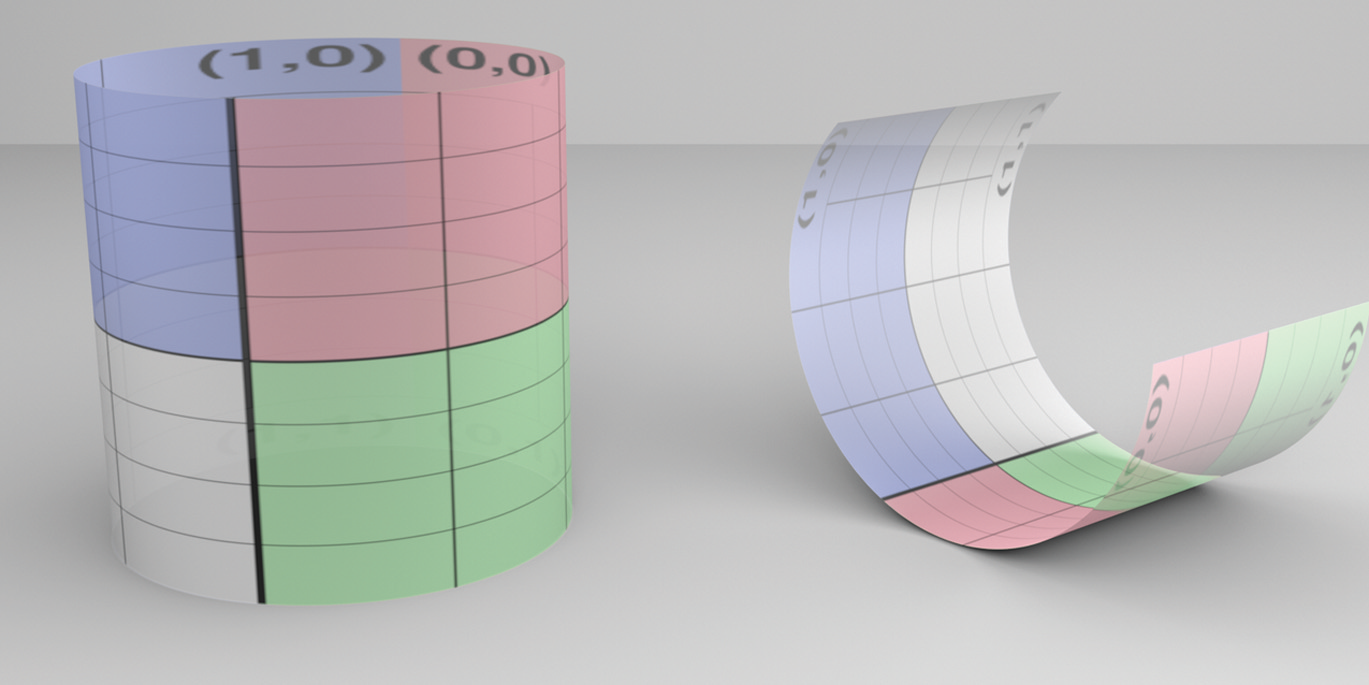
\includegraphics[width=\linewidth]{chap03/twocylinders.png}
    \caption{两个圆柱体。左边是完整圆柱体,右边是部分圆柱体。}
    \label{fig:3.7}
\end{figure}

\begin{lstlisting}
`\initcode{Cylinder Public Methods}{=}`
`\refvar{Cylinder}{}`(const `\refvar{Transform}{}` *ObjectToWorld, const `\refvar{Transform}{}` *WorldToObject,
         bool reverseOrientation, `\refvar{Float}{}` radius, `\refvar{Float}{}` zMin, `\refvar{Float}{}` zMax,
         `\refvar{Float}{}` phiMax)
    : `\refvar{Shape}{}`(ObjectToWorld, WorldToObject, reverseOrientation),
      `\refvar[Cylinder::radius]{radius}{}`(radius), `\refvar[Cylinder::zMin]{zMin}{}`(std::min(zMin, zMax)),
      `\refvar[Cylinder::zMax]{zMax}{}`(std::max(zMin, zMax)),
      `\refvar[Cylinder::phiMax]{phiMax}{}`(`\refvar{Radians}{}`(`\refvar{Clamp}{}`(phiMax, 0, 360))) { }
\end{lstlisting}
\begin{lstlisting}
`\initcode{Cylinder Private Data}{=}`
const `\refvar{Float}{}` `\initvar[Cylinder::radius]{radius}{}`, `\initvar[Cylinder::zMin]{zMin}{}`, `\initvar[Cylinder::zMax]{zMax}{}`, `\initvar[Cylinder::phiMax]{phiMax}{}`;
\end{lstlisting}

\subsection{边界}\label{sub:边界3}
像球那样,圆柱体边界方法用$z$的范围计算保守边界框但不考虑最大的$\varphi$。
\begin{lstlisting}
`\initcode{Cylinder Method Definitions}{=}\initnext{CylinderMethodDefinitions}`
`\refvar{Bounds3f}{}` `\refvar{Cylinder}{}`::`\initvar[Cylinder::ObjectBound]{\refvar{ObjectBound}{}}{}`() const {
    return `\refvar{Bounds3f}{}`(`\refvar{Point3f}{}`(-`\refvar[Cylinder::radius]{radius}{}`, -`\refvar[Cylinder::radius]{radius}{}`, `\refvar[Cylinder::zMin]{zMin}{}`),
                    `\refvar{Point3f}{}`( `\refvar[Cylinder::radius]{radius}{}`,  `\refvar[Cylinder::radius]{radius}{}`, `\refvar[Cylinder::zMax]{zMax}{}`));
}
\end{lstlisting}

\subsection{相交测试}\label{sub:相交测试3}
光线-圆柱体相交公式可以通过把射线方程代入圆柱体的隐式方程得到,和球体的情况一样。
以$z$轴为中心$r$为半径的无限长圆柱体的隐式方程为
\begin{align*}
    x^2+y^2-r^2=0\, .
\end{align*}
代入射线方程\refeq{2.3},我们有
\begin{align*}
    (o_x+td_x)^2+(o_y+td_y)^2=r^2\, .
\end{align*}
我们将其展开并求二次式方程$at^2+bt+c=0$的系数得
\begin{align*}
    a & =d_x^2+d_y^2\, ,      \\
    b & =2(d_xo_x+d_yo_y)\, , \\
    c & =o_x^2+o_y^2-r^2\, .
\end{align*}
\begin{lstlisting}
`\initcode{Compute quadratic cylinder coefficients}{=}`
`\refcode{Initialize EFloat ray coordinate values}{}`
`\refvar{EFloat}{}` a = dx * dx + dy * dy;
`\refvar{EFloat}{}` b = 2 * (dx * ox + dy * oy);
`\refvar{EFloat}{}` c = ox * ox + oy * oy - `\refvar{EFloat}{}`(`\refvar[Cylinder::radius]{radius}{}`) * `\refvar{EFloat}{}`(`\refvar[Cylinder::radius]{radius}{}`);
\end{lstlisting}

所有二次曲面形状求解二次方程的过程都一样,
所以下面会复用来自\refvar{Sphere}{}
相交方法的一些代码片。
\begin{lstlisting}
`\refcode{Cylinder Method Definitions}{+=}\lastnext{CylinderMethodDefinitions}`
bool `\refvar{Cylinder}{}`::`\initvar[Cylinder::Intersect]{\refvar[Shape::Intersect]{Intersect}{}}{}`(const `\refvar{Ray}{}` &r, `\refvar{EFloat}{}` *tHit,
        `\refvar{SurfaceInteraction}{}` *isect, bool testAlphaTexture) const {
    `\refvar{Float}{}` phi;
    `\refvar{Point3f}{}` pHit;
    `\refcode{Transform Ray to object space}{}`
    `\refcode{Compute quadratic cylinder coefficients}{}`
    `\refcode{Solve quadratic equation for t values}{}`
    `\refcode{Compute cylinder hit point and $\varphi$}{}`
    `\refcode{Test cylinder intersection against clipping parameters}{}`
    `\refcode{Find parametric representation of cylinder hit}{}`
    `\refcode{Compute error bounds for cylinder intersection}{}`
    `\refcode{Initialize SurfaceInteraction from parametric information}{}`
    `\refcode{Update tHit for quadric intersection}{}`
    return true;
}
\end{lstlisting}

像球体那样,这里的实现改进了计算的交点
以降低在计算射线方程中累积舍入误差的影响;见\refsub{定界交点误差}。
于是我们由圆柱体的参数化描述从$x$和$y$反解出$\varphi$;
最后所得结果与球体相同。
\begin{lstlisting}
`\initcode{Compute cylinder hit point and $\varphi$}{=}`
pHit = ray((`\refvar{Float}{}`)tShapeHit);
`\refcode{Refine cylinder intersection point}{}`
phi = std::atan2(pHit.y, pHit.x);
if (phi < 0) phi += 2 * `\refvar{Pi}{}`;
\end{lstlisting}

相交方法下一部分保证命中点在指定$z$范围内且能接受角度$\varphi$。
否则它就拒绝该命中点,并在之前还没尝试的前提下检查$t_1$——这和
\refvar{Sphere::Intersect}{()}
中的条件逻辑很像。
\begin{lstlisting}
`\initcode{Test cylinder intersection against clipping parameters}{=}`
if (pHit.z < `\refvar[Cylinder::zMin]{zMin}{}` || pHit.z > `\refvar[Cylinder::zMax]{zMax}{}` || phi > `\refvar[Cylinder::phiMax]{phiMax}{}`) {
    if (tShapeHit == t1) return false;
    tShapeHit = t1;
    if (t1.`\refvar{UpperBound}{}`() > ray.`\refvar{tMax}{}`) return false;
    `\refcode{Compute cylinder hit point and $\varphi$}{}`
    if (pHit.z < `\refvar[Cylinder::zMin]{zMin}{}` || pHit.z > `\refvar[Cylinder::zMax]{zMax}{}` || phi > `\refvar[Cylinder::phiMax]{phiMax}{}`)
        return false;
}
\end{lstlisting}

再次将$\varphi$缩放到0到1计算$u$值。
直接反解圆柱体参数方程的$z$值求得$v$参数坐标。
\begin{lstlisting}
`\initcode{Find parametric representation of cylinder hit}{=}`
`\refvar{Float}{}` u = phi / `\refvar[Cylinder::phiMax]{phiMax}{}`;
`\refvar{Float}{}` v = (pHit.z - `\refvar[Cylinder::zMin]{zMin}{}`) / (`\refvar[Cylinder::zMax]{zMax}{}` - `\refvar[Cylinder::zMin]{zMin}{}`);
`\refcode{Compute cylinder $\partial$p/$\partial$u and $\partial$p/$\partial$v}{}`
`\refcode{Compute cylinder $\partial$n/$\partial$u and $\partial$n/$\partial$v}{}`
\end{lstlisting}

圆柱体的偏导数很容易推导:
\begin{align*}
    \frac{\partial\bm p}{\partial u} & =(-\varphi_{\max}y,\varphi_{\max}x,0)\, , \\
    \frac{\partial\bm p}{\partial v} & =(0,0,z_{\max}-z_{\min})\, .
\end{align*}
\begin{lstlisting}
`\initcode{Compute cylinder $\partial$p/$\partial$u and $\partial$p/$\partial$v}{=}`
`\refvar{Vector3f}{}` dpdu(-`\refvar[Cylinder::phiMax]{phiMax}{}` * pHit.y, `\refvar[Cylinder::phiMax]{phiMax}{}` * pHit.x, 0);
`\refvar{Vector3f}{}` dpdv(0, 0, `\refvar[Cylinder::zMax]{zMax}{}` - `\refvar[Cylinder::zMin]{zMin}{}`);
\end{lstlisting}

我们又用外恩加滕方程计算圆柱法线的参数化偏导数。
相关偏导数为:
\begin{align*}
    \frac{\partial^2\bm p}{\partial u^2}         & =-\varphi_{\max}^2(x,y,0)\, , \\
    \frac{\partial^2\bm p}{\partial u\partial v} & =(0,0,0)\, ,                  \\
    \frac{\partial^2\bm p}{\partial v^2}         & =(0,0,0)\, .
\end{align*}
\begin{lstlisting}
`\initcode{Compute cylinder $\partial$n/$\partial$u and $\partial$n/$\partial$v}{=}`
`\refvar{Vector3f}{}` d2Pduu = -`\refvar[Cylinder::phiMax]{phiMax}{}` * `\refvar[Cylinder::phiMax]{phiMax}{}` * `\refvar{Vector3f}{}`(pHit.x, pHit.y, 0);
`\refvar{Vector3f}{}` d2Pduv(0, 0, 0), d2Pdvv(0, 0, 0);
`\refcode{Compute coefficients for fundamental forms}{}`
`\refcode{Compute $\partial$n/$\partial$u and $\partial$n/$\partial$v from fundamental form coefficients}{}`
\end{lstlisting}

\subsection{表面积}\label{sub:表面积3}
圆柱体就是卷起来的矩形。如果你展开矩形,
其高是$z_{\max}-z_{\min}$,宽是$r\varphi_{\max}$:
\begin{lstlisting}
`\refcode{Cylinder Method Definitions}{+=}\lastnext{CylinderMethodDefinitions}`
`\refvar{Float}{}` `\refvar{Cylinder}{}`::`\initvar[Cylinder::Area]{\refvar[Shape::Area]{Area}{}}{}`() const {
    return (`\refvar[Cylinder::zMax]{zMax}{}` - `\refvar[Cylinder::zMin]{zMin}{}`) * `\refvar[Cylinder::radius]{radius}{}` * `\refvar[Cylinder::phiMax]{phiMax}{}`;
}
\end{lstlisting}